\section{Příklad 1}
\prvniZadani{F}

\begin{enumerate}
    \item \textbf{Seriové zapojení zdroju $U_1$, $U_2$:} \newline
    $U_{12} = U_1 + U_2 = 125V + 65V = 190V$
    
    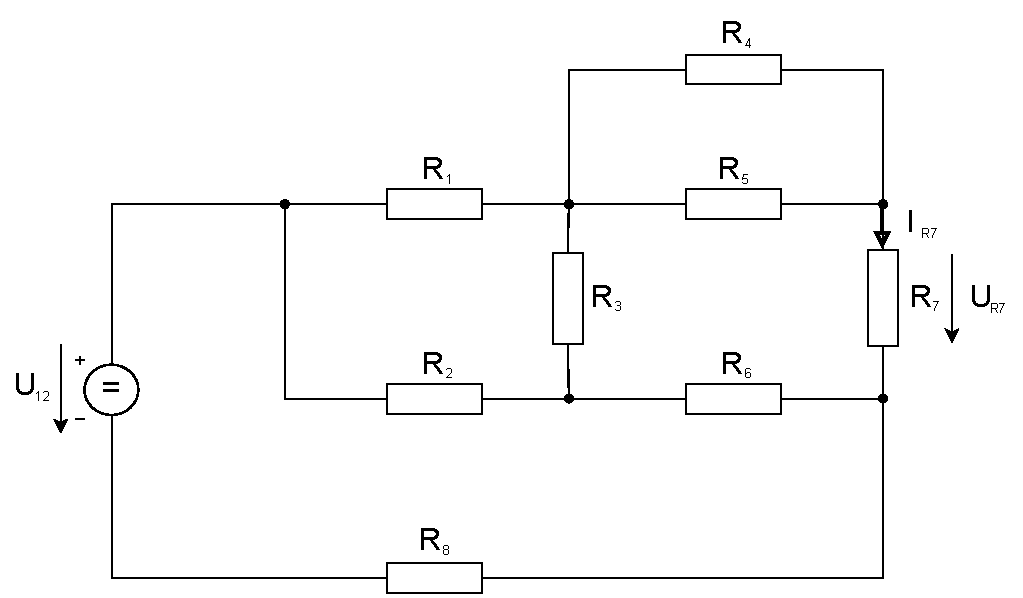
\includegraphics[scale=0.7]{pr1/pr1.1pdf.pdf}
    
    \item \textbf{Paralelní zapojení rezistorů $R_4$, $R_5$:} \newline $R_{45} = \frac{R_4 * R_5}{R_4 + R_5} = \frac{250\Omega * 300\Omega}{250\Omega + 300\Omega} = \frac{75000\Omega}{550\Omega} = 136,3636\Omega$
    
    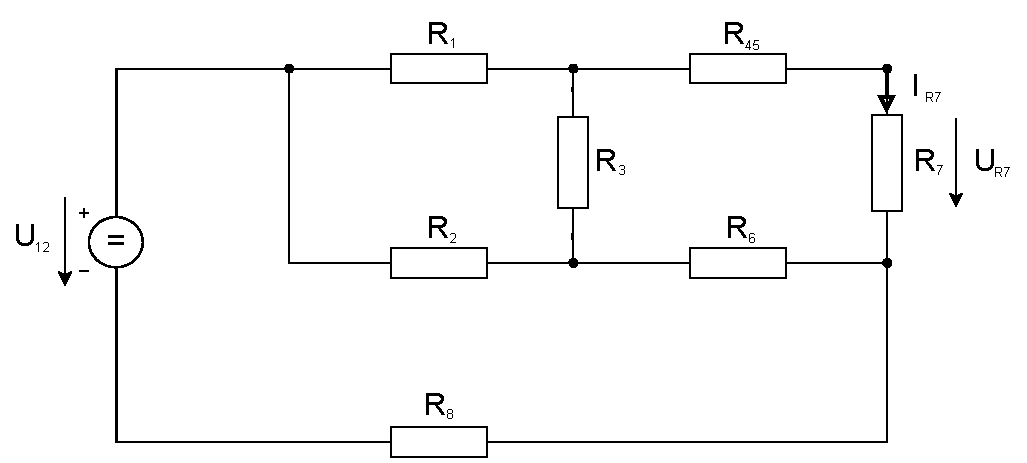
\includegraphics[scale=0.7]{pr1/pr1.2.pdf}
    
    \item \textbf{Seriové zapojení rezistorů $R_{45}$, $R_7$:} \newline
    $R_{457} = R_{45} + R_7 = 136,3636\Omega + 330\Omega = 466,3636\Omega$
    
    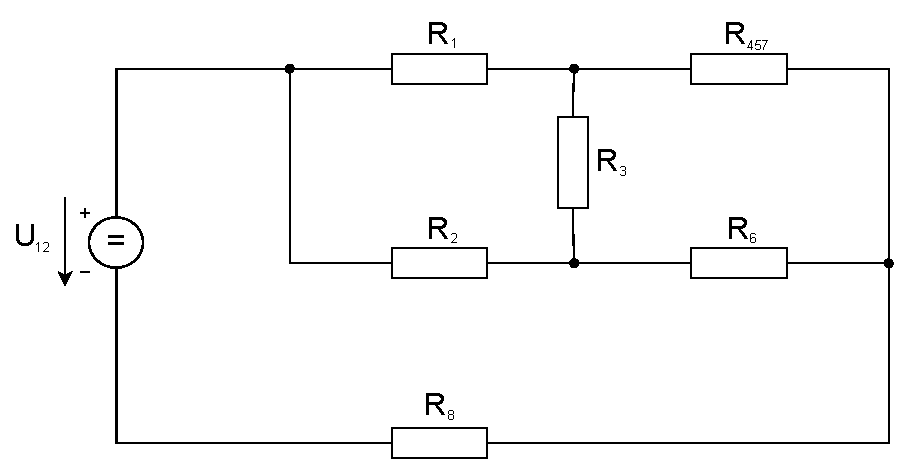
\includegraphics[scale=0.7]{pr1/pr1.3.pdf}
 
    \item \textbf{Trojůhelnik - Hvězda:} \newline
    $R_A = \frac{R_1 * R_2}{R_1 + R_2 + R_3} = \frac{510\Omega * 500\Omega}{510\Omega + 500\Omega + 550\Omega} = \frac{255000\Omega}{1560\Omega} = 163,4615\Omega$ \newline
 
    $R_B = \frac{R_1 * R_3}{R_1 + R_2 + R_3} = \frac{510\Omega * 550\Omega}{510\Omega + 500\Omega + 550\Omega} = \frac{280500\Omega}{1560\Omega} = 179,8007\Omega$ \newline

    $R_C = \frac{R_2 * R_3}{R_1 + R_2 + R_3} = \frac{500\Omega * 550\Omega}{510\Omega + 500\Omega + 550\Omega} = \frac{275000\Omega}{1560\Omega} = 176,2820\Omega$ \newline
    
    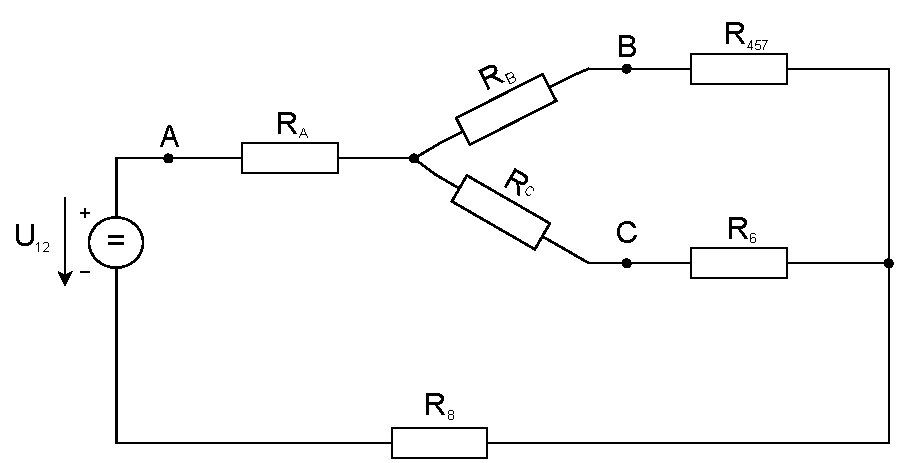
\includegraphics[scale=0.7]{pr1/pr1.4.pdf}
  
    \item \textbf{Seriové zapojení rezistorů $R_B$, $R_{457}$:} \newline
    $R_{B457} = R_B + R_{457} = 179,8077\Omega + 466,3636\Omega = 646,1643\Omega$

    \item \textbf{Seriové zapojení rezistorů $R_C$, $R_6$:} \newline
    $R_{C6} = R_C + R_6 = 176,2820\Omega + 800\Omega = 976,2820\Omega$
    
    \begin{center}
    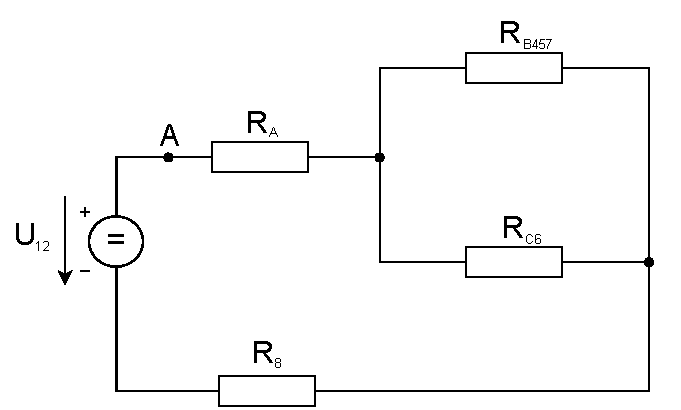
\includegraphics[scale=0.7]{pr1/pr1.5.pdf}
    \end{center}
  
    \item \textbf{Paralelní zapojení rezistorů $R_{B457}$, $R_{C6}$:} \newline
    $R_{BC4567} = \frac{R_{B457} * R_{C6}}{R_{B457} + R_{C6}} = \frac{646,1643\Omega * 976,2820\Omega}{646,1643\Omega + 976,2820\Omega} = \frac{630838,5751\Omega}{1622,4463\Omega} = 388,8194\Omega$
    
    \begin{center}
    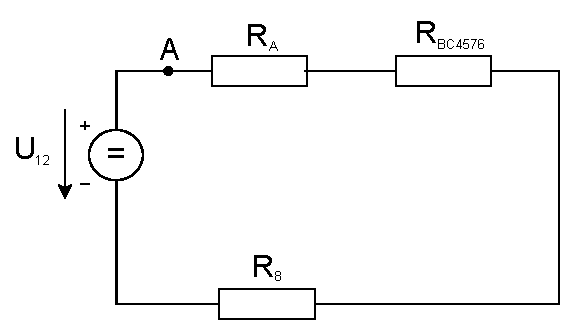
\includegraphics[scale=0.7]{pr1/pr1.6.pdf}
    \end{center}
    
    \item \textbf{Seriové zapojení rezistorů $R_A$, $R_{BC4567}$, $R_8$:} \newline
    $R_{EKV} = R_A + R_{BC4567} + R_8 = 163,4615\Omega + 388,8194\Omega + 250\Omega = 802,2809\Omega$
    
    \begin{center}
    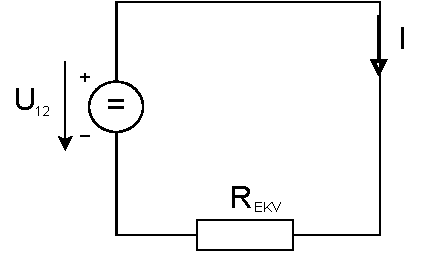
\includegraphics[scale=0.7]{pr1/pr1.7.pdf}
    \end{center}

    \item \textbf{Proud obvodu:} \newline
    $I = \frac{U_{12}}{R_{EKV}} = \frac{190V}{802,2809\Omega} = 0,2368A$
  
    \item \textbf{Napětí $R_{BC4567}$:} \newline
    $U_{RBC4567} = I * R_{BC4567} = 0,2368A * 388,8194\Omega = 92,0724V$
    
    \item \textbf{Proud $I_{R7}$:} \newline
    $I_{R7} = I_{RB457} = \frac{U_{RBC4567}}{R_{B457}} = \frac{92,0724V}{646,1643\Omega} = 0,1425A$
    
    \item \textbf{Napětí $U_{R7}$:} \newline
    $U_{R7} = I_{R7} * R_7 = 0,1425A * 330\Omega = 47,025V$
\end{enumerate}

